\section{Auswertung}
\label{sec:Auswertung}

\subsection{Bestimmung von $U_0$ und $R_i$ der Monozelle}

Es wird die Klemmspannung $U_k$ in Abhängigkeit des Stromes $I$ gemessen. 
Die aufgenommenen Werte sind in Tabelle \ref{tab:Monozelle} aufgeführt. 

\begin{table}
\centering
\caption{Spannungs- und Stromwerte der Monozelle}
\label{tab:Monozelle}
\sisetup{table-format=2.1}
\begin{tabular}{c c}
\toprule
$U_k \,/\, \si{\volt}$ & $I \,/\, \si{\milli\ampere}$\\
\midrule
1.550 & 25.0\\
1.525 &  27.5\\
1.500 &  31.0\\
1.450 &  38.0\\
1.425 &  46.0\\
1.400 &  49.5\\
1.350 &  57.0\\
1.300 &  61.5\\
1.250 &  77.5\\
1.200 &  85.0\\
1.100 & 110.0\\
0.700 & 175.0\\
0.450 & 215.0\\
0.400 & 225.0\\
\bottomrule
\end{tabular}
\end{table}



\begin{figure}
  \centering
  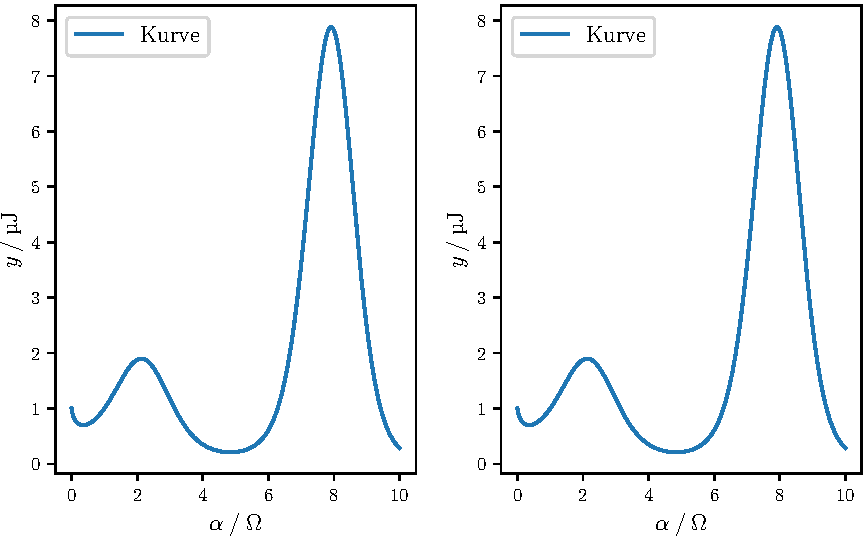
\includegraphics{plot.pdf}
  \caption{Plot.}
  \label{fig:plot}
\end{figure}
